\documentclass{article}
% \VignettePackage{adegenet-genomics}
% \VignetteIndexEntry{Analysing genome-wide SNP data using adegenet}

\usepackage{graphicx}
\usepackage[colorlinks=true,urlcolor=blue]{hyperref}
\usepackage{array}
\usepackage{color}

\usepackage[utf8]{inputenc} % for UTF-8/single quotes from sQuote()
\newcommand{\code}[1]{{{\tt #1}}}
\title{Analysing genome-wide SNP data using  \textit{adegenet} 1.3-0}
\author{Thibaut Jombart}
\date{\today}




\sloppy
\hyphenpenalty 10000


\usepackage{Sweave}
\begin{document}





\definecolor{Soutput}{rgb}{0,0,0.56}
\definecolor{Sinput}{rgb}{0.56,0,0}
\DefineVerbatimEnvironment{Sinput}{Verbatim}
{formatcom={\color{Sinput}},fontsize=\footnotesize, baselinestretch=0.75}
\DefineVerbatimEnvironment{Soutput}{Verbatim}
{formatcom={\color{Soutput}},fontsize=\footnotesize, baselinestretch=0.75}

\color{black}

\maketitle

\begin{abstract}
  Genome-wide SNP data can quickly be challenging to analyse using standard
  computer. The package \textit{adegenet} \cite{tjart05} for the R software \cite{np145}
  implements representation of these data with unprecedented efficiency
  using the classes \texttt{SNPbin} and \texttt{genlight}, which can require up to 60 times less RAM than usual
  representation using allele frequencies.
  This vignette introduces these classes and illustrates how these objects can be handled and
  analyzed in R.
  It also introduces more advanced features of an API in C language which may be useful to develop
  new method based on these objects.
\end{abstract}

\newpage

\tableofcontents


\newpage
%%%%%%%%%%%%%%%%
%%%%%%%%%%%%%%%%
\section{Introduction}
%%%%%%%%%%%%%%%%
%%%%%%%%%%%%%%%%
Modern sequencing technologies now make complete genomes more widely accessible.
The subsequent amounts of genetic data pose challenges in terms of storing and handling the data,
making former tools developed for classical genetic markers such as microsatellite impracticable using
standard computers.
Adegenet has developed new object classes dedicated to handling genome-wide polymorphism (SNPs) with
minimum rapid access memory (RAM) requirements.
\\

Two new formal classes have been implemented: \texttt{SNPbin}, used to store genome-wide SNPs for
one individual, and \texttt{genlight}, which stored the same information for multiple individuals.
Information represented this way is binary: only biallelic SNPs can be stored and analyzed using these classes.
However, these objects are otherwise very flexible, and can incorporate different levels of ploidy
across individuals within a single dataset.
In this vignette, we present these object classes and show how their content can be further handled and
content analyzed.





%%%%%%%%%%%%%%%%
%%%%%%%%%%%%%%%%
\section{Classes of objects}
%%%%%%%%%%%%%%%%
%%%%%%%%%%%%%%%%

%%%%%%%%%%%%%%%%
\subsection{\code{SNPbin}: storage of single genomes}
%%%%%%%%%%%%%%%%
The class \texttt{SNPbin} is the core representation of biallelic SNPs which allows to represent
data with unprecedented efficiency.
The essential idea is to code binary SNPs not as integers, but as bits. This operation is tricky in
R as there is no handling of bits, only bytes -- series of 8 bits. However, the class
\texttt{SNPbin} handles this transparently using sub-rountines in C language.
Considerable efforts have been made so that the user does not have to dig into the complex internal
structure of the objects, and can handle \texttt{SNPbin} objects as easily as possible.
\\

Like \texttt{genind} and \texttt{genpop} objects, \texttt{SNPbin} is a formal "S4" class. The
structure of these objects is detailed in the dedicated manpage (\texttt{?SNPbin}). As all S4
objects, instances of the class \texttt{SNPbin} are composed of slots accessible using the
\texttt{@} operator. This content is generic (it is the same for all instances of the class), and returned by:
\begin{Schunk}
\begin{Sinput}
> library(adegenet)
> getClassDef("SNPbin")
\end{Sinput}
\begin{Soutput}
Class "SNPbin" [package "adegenet"]

Slots:
                                                             
Name:         snp      n.loc    NA.posi      label     ploidy
Class:       list    integer    integer charOrNULL    integer
\end{Soutput}
\end{Schunk}

The slots respectively contain:
\begin{itemize}
  \item \texttt{snp}: SNP data with specific internal coding.
  \item \texttt{n.loc}: the number of SNPs stored in the object.
  \item \texttt{NA.posi}: position of the missing data (NAs).
  \item \texttt{label}: an optional label for the individual.
  \item \texttt{ploidy}: the ploidy level of the genome.
\end{itemize}

New objects are created using \texttt{new}, with these slots as arguments.
If no argument is provided, an empty object is created:
\begin{Schunk}
\begin{Sinput}
> new("SNPbin")
\end{Sinput}
\begin{Soutput}
 === S4 class SNPbin ===
 0 SNPs coded as bits
 Ploidy: 1
 0 (NaN %) missing data
\end{Soutput}
\end{Schunk}
In practice, only the \texttt{snp} information and possibly the ploidy has to be provided; various
formats are accepted for the \texttt{snp} component, but the simplest is a vector of integers (or
numeric) indicating the number of second allele at each locus.
The argument \texttt{snp}, if provided alone, does not have to be named:
\begin{Schunk}
\begin{Sinput}
> x <- new("SNPbin", c(0, 1, 1, 2, 0, 0, 1))
> x
\end{Sinput}
\begin{Soutput}
 === S4 class SNPbin ===
 7 SNPs coded as bits
 Ploidy: 2
 0 (0 %) missing data
\end{Soutput}
\end{Schunk}

If not provided, the ploidy is detected from the data and determined as the largest number in the
input vector. Obviously, in many cases this will not be adequate, but ploidy can always be rectified
afterwards; for instance:
\begin{Schunk}
\begin{Sinput}
> x
\end{Sinput}
\begin{Soutput}
 === S4 class SNPbin ===
 7 SNPs coded as bits
 Ploidy: 2
 0 (0 %) missing data
\end{Soutput}
\begin{Sinput}
> ploidy(x) <- 3
> x
\end{Sinput}
\begin{Soutput}
 === S4 class SNPbin ===
 7 SNPs coded as bits
 Ploidy: 3
 0 (0 %) missing data
\end{Soutput}
\end{Schunk}

\noindent The internal coding of the objects is cryptic, and not meant to be accessed directly:
\begin{Schunk}
\begin{Sinput}
> x@snp
\end{Sinput}
\begin{Soutput}
[[1]]
[1] 08

[[2]]
[1] 4e
\end{Soutput}
\end{Schunk}
Fortunately, data are easily converted back into integers:
\begin{Schunk}
\begin{Sinput}
> as.integer(x)
\end{Sinput}
\begin{Soutput}
[1] 0 1 1 2 0 0 1
\end{Soutput}
\end{Schunk}

~\\

The main interest of this representation is its efficiency in terms of storage.
For instance:
\begin{Schunk}
\begin{Sinput}
> dat <- sample(0:1, 1e+06, replace = TRUE)
> print(object.size(dat), unit = "auto")
\end{Sinput}
\begin{Soutput}
3.8 Mb
\end{Soutput}
\begin{Sinput}
> x <- new("SNPbin", dat)
> print(object.size(x), unit = "auto")
\end{Sinput}
\begin{Soutput}
123.4 Kb
\end{Soutput}
\end{Schunk}
here, we converted a million SNPs into a \texttt{SNPbin} object, which turns out to be
32 smaller than the original data.
However, the information in \texttt{dat} and \texttt{x} is strictly identical:
\begin{Schunk}
\begin{Sinput}
> identical(as.integer(x), dat)
\end{Sinput}
\begin{Soutput}
[1] TRUE
\end{Soutput}
\end{Schunk}
The advantage of this storage is therefore being extremely compact, and allowing to analyse big
datasets using standard computers.
%% Obviously, usual computations demand data to be at one moment coded as numeric values (as opposed to bits).
%% However in most cases, we can proceed by only converting one or two genomes back to numeric values
%% at a time, therefore keeping RAM requirements low, albeit at a possible increase in computational time.
%% This however is minimized by two ways: i) conversion routines are optimized for speed using C code
%% ii) smaller objects are handled, therefore decreasing the possibly high computational time taken by memory allocation.
\\

While \texttt{SNPbin} objects are the very mean by which we store data efficiently, in practice
we need to analyze several genomes at a time.
This is made possible by the class \texttt{genlight}, which relies on \texttt{SNPbin} but allows for
storing data from several genomes at a time.




%%%%%%%%%%%%%%%%
\subsection{\code{genlight}: storage of multiple genomes}
%%%%%%%%%%%%%%%%

Like \texttt{SNPbin}, \texttt{genlight} is a formal S4 class.
The slots of instances of this class are described by:
\begin{Schunk}
\begin{Sinput}
> getClassDef("genlight")
\end{Sinput}
\begin{Soutput}
Class "genlight" [package "adegenet"]

Slots:
                                                                       
Name:           gen        n.loc    ind.names    loc.names      loc.all
Class:         list      integer   charOrNULL   charOrNULL   charOrNULL
                                                                       
Name:    chromosome     position       ploidy          pop        other
Class: factorOrNULL    intOrNULL    intOrNULL factorOrNULL         list
\end{Soutput}
\end{Schunk}
As it can be seen, these objects allow for storing more information in addition to vectors of SNP frequencies.
More precisely, their content is (see \texttt{?genlight} for more details):
\begin{itemize}
  \item \texttt{gen}: SNP data for different individuals, each stored as a \texttt{SNPbin}; loci
    have to be identical across all individuals.
  \item \texttt{n.loc}: the number of SNPs stored in the object.
  \item \texttt{ind.names}: (optional) labels for the individuals.
  \item \texttt{loc.names}: (optional) labels for the loci.
  \item \texttt{loc.all}: (optional) alleles of the loci separated by '/' (e.g. 'a/t', 'g/c', etc.).
  \item \texttt{chromosome}: (optional) a factor indicating the chromosome to which the SNPs belong.
  \item \texttt{position}: (optional) the position of each SNPs in their chromosome.
  \item \texttt{ploidy}: (optional) the ploidy of each individual.
  \item \texttt{pop}: (optional) a factor grouping individuals into 'populations'.
  \item \texttt{other}: (optional) a list containing any supplementary information to be stored with
    the data.
\end{itemize}

\noindent Like \texttt{SNPbin} object, \texttt{genlight} object are created using the constructor \texttt{new},
providing content for the slots above as arguments.
When none is provided, an empty object is created:
\begin{Schunk}
\begin{Sinput}
> new("genlight")
\end{Sinput}
\begin{Soutput}
 === S4 class genlight ===
 0 genotypes,  0 binary SNPs
\end{Soutput}
\end{Schunk}
The most important information to provide is obviously the genotypes (argument \texttt{gen}); these
can be provided as:
\begin{itemize}
\item a \texttt{list} of integer vectors representing the number of second allele at each locus.
\item a \texttt{matrix} / \texttt{data.frame} of integers, with individuals in rows and SNPs in columns.
\item a list of \texttt{SNPbin} objects.
\end{itemize}

Ploidy has to be consistent across loci for a given individual, but individuals do not have to have
the same ploidy, so that it is possible to have hapoid,
diploid, and tetraploid individuals in the same dataset; for instance:
\begin{Schunk}
\begin{Sinput}
> x <- new("genlight", list(indiv1 = c(1, 1, 0, 1, 1, 0), indiv2 = c(2, 
+     1, 1, 0, 0, 0), toto = c(2, 2, 0, 0, 4, 4)))
> x
\end{Sinput}
\begin{Soutput}
 === S4 class genlight ===
 3 genotypes,  6 binary SNPs
 Ploidy statistics (min/median/max): 1 / 2 / 4
 0 (0 %) missing data
\end{Soutput}
\begin{Sinput}
> ploidy(x)
\end{Sinput}
\begin{Soutput}
indiv1 indiv2   toto 
     1      2      4 
\end{Soutput}
\end{Schunk}

As for \texttt{SNPbin}, \texttt{genlight} objects can be converted back to integers vectors, stored
as matrices or lists:
\begin{Schunk}
\begin{Sinput}
> as.list(x)
\end{Sinput}
\begin{Soutput}
$indiv1
[1] 1 1 0 1 1 0

$indiv2
[1] 2 1 1 0 0 0

$toto
[1] 2 2 0 0 4 4
\end{Soutput}
\begin{Sinput}
> as.matrix(x)
\end{Sinput}
\begin{Soutput}
       [,1] [,2] [,3] [,4] [,5] [,6]
indiv1    1    1    0    1    1    0
indiv2    2    1    1    0    0    0
toto      2    2    0    0    4    4
\end{Soutput}
\end{Schunk}

\noindent In practice, \texttt{genlight} objects can be handled as if they were matrices of integers
as the one above returned by \texttt{as.matrix}.
However, they offer the advantage of efficient storage of the information; for instance, we can
simulate 50 individuals typed for 1,00,000 SNPs each (including occasional NAs):
\begin{Schunk}
\begin{Sinput}
> dat <- lapply(1:50, function(i) sample(c(0, 1, NA), 1e+06, prob = c(0.5, 
+     0.499, 0.001), replace = TRUE))
> names(dat) <- paste("indiv", 1:length(dat))
> print(object.size(dat), unit = "auto")
\end{Sinput}
\begin{Soutput}
381.5 Mb
\end{Soutput}
\begin{Sinput}
> x <- new("genlight", dat)
> print(object.size(x), unit = "auto")
\end{Sinput}
\begin{Soutput}
6.2 Mb
\end{Soutput}
\begin{Sinput}
> object.size(dat)/object.size(x)
\end{Sinput}
\begin{Soutput}
61.3365722669428 bytes
\end{Soutput}
\end{Schunk}
here again, the storage if the data is much more efficient in \texttt{genlight} than using integers: converted data occupy
61 times less memory than the original data.
\\

The advantage of this storage is therefore being extremely compact, and allowing to analyse very large
datasets using standard computers.
Obviously, usual computations demand data to be at one moment coded as numeric values (as opposed to bits).
However, most usual computations can be achieved by only converting one or two genomes back to numeric values
at a time, therefore keeping RAM requirements low, albeit at a possible cost of increased computational time.
This however is minimized by three ways:
\begin{enumerate}
\item conversion routines are optimized for speed using C code.
\item using parallel computation where multicore architectures are available.
\item handling smaller objects, thereby decreasing the possibly high computational time taken by memory allocation.
\end{enumerate}

While this makes implementing methods more complicated.
In practice, routines are implemented so as to minimize
the amount of data converted back to integers, use C code where possible, and use multiple cores
if the package \textit{multicore} is installed an multiple cores are available.
Fortunately, these underlying technical issues are oblivious to the user, and one merely needs to
know how to manipulate \texttt{genlight} objects using a few key functions to be able to analyze data.






%%%%%%%%%%%%%%%%
%%%%%%%%%%%%%%%%
\section{Data handling using \texttt{genlight} objects}
%%%%%%%%%%%%%%%%
%%%%%%%%%%%%%%%%

%%%%%%%%%%%%%%%%
\subsection{Using accessors}
%%%%%%%%%%%%%%%%

In the following, we demonstrate how to manipulate and analyse \texttt{genlight} objects.
The phylosophy underlying formal (S4) classes in general, and \texttt{genlight} objects in
particular, is that internal representation of the information can be complex as long as accessing
this information is simple.
This is made possible by decoupling storage and accession: the user is not meant to access the
content of the object directly, but has to use \texttt{accessors} to retrieve or modify information.
\\

Available accessors are documented in \code{?genlight}.
Most of them are identical to accessors for \texttt{genind} and \texttt{genpop} objects, such as:
\begin{itemize}
  \item \texttt{nInd}: returns the number of individuals in the object.
  \item \texttt{nLoc}: returns the number of loci (SNPs).
  \item \texttt{indNames}$^{\dagger}$: returns/sets labels for individuals.
  \item \texttt{locNames}$^{\dagger}$: returns/sets labels for loci (SNPs).
  \item \texttt{alleles}$^{\dagger}$: returns/sets alleles.
  \item \texttt{ploidy}$^{\dagger}$: returns/sets ploidy of the individuals.
  \item \texttt{pop}$^{\dagger}$: returns/sets a factor grouping individuals.
  \item \texttt{other}$^{\dagger}$: returns/sets misc information stored as a list.
\end{itemize}
where $^{\dagger}$ indicates that a replacement method is available using \texttt{<-'}; for instance:
\begin{Schunk}
\begin{Sinput}
> dat <- lapply(1:3, function(i) sample(0:2, 10, replace = TRUE))
> dat
\end{Sinput}
\begin{Soutput}
[[1]]
 [1] 1 0 1 2 1 0 0 0 1 2

[[2]]
 [1] 0 1 0 0 0 2 1 1 1 0

[[3]]
 [1] 2 0 1 2 0 0 2 2 1 1
\end{Soutput}
\begin{Sinput}
> x <- new("genlight", dat)
> x
\end{Sinput}
\begin{Soutput}
 === S4 class genlight ===
 3 genotypes,  10 binary SNPs
 Ploidy: 2
 0 (0 %) missing data
\end{Soutput}
\begin{Sinput}
> indNames(x)
\end{Sinput}
\begin{Soutput}
NULL
\end{Soutput}
\begin{Sinput}
> indNames(x) <- paste("individual", 1:3)
> indNames(x)
\end{Sinput}
\begin{Soutput}
[1] "individual 1" "individual 2" "individual 3"
\end{Soutput}
\begin{Sinput}
> locNames(x)
> locNames(x) <- paste("SNP", 1:nLoc(x), sep = ".")
> as.matrix(x)
\end{Sinput}
\begin{Soutput}
             SNP.1 SNP.2 SNP.3 SNP.4 SNP.5 SNP.6 SNP.7 SNP.8 SNP.9 SNP.10
individual 1     1     0     1     2     1     0     0     0     1      2
individual 2     0     1     0     0     0     2     1     1     1      0
individual 3     2     0     1     2     0     0     2     2     1      1
\end{Soutput}
\end{Schunk}

\noindent
In addition, some specific accessors are available for \texttt{genlight} objects:
\begin{itemize}
  \item \texttt{NA.posi}: returns the position of missing values in each individual.
  \item \texttt{chromosome}$^{\dagger}$: returns/sets the chromosome of each SNP.
  \item \texttt{chr}$^{\dagger}$: same as \texttt{chromosome} --- used as a shortcut.
  \item \texttt{position}$^{\dagger}$: returns/sets the position of each SNP.
\end{itemize}


Accessors are meant to be clever about replacement, meaning that they try hard to prevent
replacement with inconsistent values. For instance, in object \texttt{x}:
\begin{Schunk}
\begin{Sinput}
> x
\end{Sinput}
\begin{Soutput}
 === S4 class genlight ===
 3 genotypes,  10 binary SNPs
 Ploidy: 2
 0 (0 %) missing data
 @loc.names: labels of the SNPs
\end{Soutput}
\end{Schunk}
if we try to set information about the chromosomes of the SNPs, the instruction:
\begin{Schunk}
\begin{Sinput}
> chr(x) <- rep("chr-1", 7)
\end{Sinput}
\end{Schunk}
will generate an error because the provided factor does not match the number of loci (10), while:
\begin{Schunk}
\begin{Sinput}
> chr(x) <- rep("chr-1", 10)
> x
\end{Sinput}
\begin{Soutput}
 === S4 class genlight ===
 3 genotypes,  10 binary SNPs
 Ploidy: 2
 0 (0 %) missing data
 @chromosome: chromosome of the SNPs
 @loc.names: labels of the SNPs
\end{Soutput}
\begin{Sinput}
> chr(x)
\end{Sinput}
\begin{Soutput}
 [1] chr-1 chr-1 chr-1 chr-1 chr-1 chr-1 chr-1 chr-1 chr-1 chr-1
Levels: chr-1
\end{Soutput}
\end{Schunk}
is a valid replacement.




%%%%%%%%%%%%%%%%
\subsection{Subsetting the data}
%%%%%%%%%%%%%%%%
\texttt{genlight} objects are meant to be handled as if they were matrices of allele numbers, as
returned by \texttt{as.matrix}.
Therefore, subsetting can be achieved using $[$ \texttt{idx.row , idx.col} $]$ where \texttt{idx.row}
and \texttt{idx.col} are indices for rows (individuals) and columns (SNPs).
For instance, using the previous toy dataset, we try a few classical subsetting of rows and columns:
\begin{Schunk}
\begin{Sinput}
> x
\end{Sinput}
\begin{Soutput}
 === S4 class genlight ===
 3 genotypes,  10 binary SNPs
 Ploidy: 2
 0 (0 %) missing data
 @chromosome: chromosome of the SNPs
 @loc.names: labels of the SNPs
\end{Soutput}
\begin{Sinput}
> as.matrix(x)
\end{Sinput}
\begin{Soutput}
             SNP.1 SNP.2 SNP.3 SNP.4 SNP.5 SNP.6 SNP.7 SNP.8 SNP.9 SNP.10
individual 1     1     0     1     2     1     0     0     0     1      2
individual 2     0     1     0     0     0     2     1     1     1      0
individual 3     2     0     1     2     0     0     2     2     1      1
\end{Soutput}
\begin{Sinput}
> as.matrix(x[c(1, 3), ])
\end{Sinput}
\begin{Soutput}
             SNP.1 SNP.2 SNP.3 SNP.4 SNP.5 SNP.6 SNP.7 SNP.8 SNP.9 SNP.10
individual 1     1     0     1     2     1     0     0     0     1      2
individual 3     2     0     1     2     0     0     2     2     1      1
\end{Soutput}
\begin{Sinput}
> as.matrix(x[, c(TRUE, FALSE)])
\end{Sinput}
\begin{Soutput}
             SNP.1 SNP.3 SNP.5 SNP.7 SNP.9
individual 1     1     1     1     0     1
individual 2     0     0     0     1     1
individual 3     2     1     0     2     1
\end{Soutput}
\begin{Sinput}
> as.matrix(x[1:2, c(1, 1, 1, 2, 2, 2, 3, 3, 3)])
\end{Sinput}
\begin{Soutput}
             SNP.1 SNP.1 SNP.1 SNP.2 SNP.2 SNP.2 SNP.3 SNP.3 SNP.3
individual 1     1     1     1     0     0     0     1     1     1
individual 2     0     0     0     1     1     1     0     0     0
\end{Soutput}
\end{Schunk}


Moreover, one can split data into blocks of SNPs using \texttt{seploc}.
This can be achieved by specifying either a number of blocks (argument \texttt{n.block}) or the size
of the blocks (argument \texttt{block.size}). The function also allows for randomizing the
distribution of the SNPs in the blocks (argument \texttt{random=TRUE}), which is especially useful
to replace computations that cannot be achieved on the whole dataset with parallelized computations performed on random blocks.
For instance:
\begin{Schunk}
\begin{Sinput}
> x
\end{Sinput}
\begin{Soutput}
 === S4 class genlight ===
 3 genotypes,  10 binary SNPs
 Ploidy: 2
 0 (0 %) missing data
 @chromosome: chromosome of the SNPs
 @loc.names: labels of the SNPs
\end{Soutput}
\begin{Sinput}
> as.matrix(x)
\end{Sinput}
\begin{Soutput}
             SNP.1 SNP.2 SNP.3 SNP.4 SNP.5 SNP.6 SNP.7 SNP.8 SNP.9 SNP.10
individual 1     1     0     1     2     1     0     0     0     1      2
individual 2     0     1     0     0     0     2     1     1     1      0
individual 3     2     0     1     2     0     0     2     2     1      1
\end{Soutput}
\begin{Sinput}
> seploc(x, n.block = 2)
\end{Sinput}
\begin{Soutput}
$block.1
 === S4 class genlight ===
 3 genotypes,  5 binary SNPs
 Ploidy: 2
 0 (0 %) missing data
 @chromosome: chromosome of the SNPs
 @loc.names: labels of the SNPs

$block.2
 === S4 class genlight ===
 3 genotypes,  5 binary SNPs
 Ploidy: 2
 0 (0 %) missing data
 @chromosome: chromosome of the SNPs
 @loc.names: labels of the SNPs
\end{Soutput}
\begin{Sinput}
> lapply(seploc(x, n.block = 2), as.matrix)
\end{Sinput}
\begin{Soutput}
$block.1
             SNP.1 SNP.2 SNP.3 SNP.4 SNP.5
individual 1     1     0     1     2     1
individual 2     0     1     0     0     0
individual 3     2     0     1     2     0

$block.2
             SNP.6 SNP.7 SNP.8 SNP.9 SNP.10
individual 1     0     0     0     1      2
individual 2     2     1     1     1      0
individual 3     0     2     2     1      1
\end{Soutput}
\end{Schunk}
splits the data into two blocks of contiguous SNPs, while:
\begin{Schunk}
\begin{Sinput}
> lapply(seploc(x, n.block = 2, random = TRUE), as.matrix)
\end{Sinput}
\begin{Soutput}
$block.1
             SNP.8 SNP.5 SNP.2 SNP.6 SNP.1
individual 1     0     1     0     0     1
individual 2     1     0     1     2     0
individual 3     2     0     0     0     2

$block.2
             SNP.4 SNP.9 SNP.10 SNP.7 SNP.3
individual 1     2     1      2     0     1
individual 2     0     1      0     1     0
individual 3     2     1      1     2     1
\end{Soutput}
\end{Schunk}
generates blocks of randomly selected SNPs.




%%%%%%%%%%%%%%%%
\subsection{Data conversions}
%%%%%%%%%%%%%%%%

% % % % % % % % % % % % %
\subsubsection{The \texttt{.snp} format}
% % % % % % % % % % % % %

\textit{adegenet} has defined its own format for storing biallelic SNP data in text files with
extension \texttt{.snp}.
This format has several advantages: it is fairly compact (more so than usual non-compressed
formats), allows for any information about individuals or loci to be stored, allows for comments,
and is easily parsed --- in particular, not all information has to be read at a time, again
minimizing RAM requirements for import procedures.


An example file of this format is distributed with adegenet.
Once the package has been installed, the file can be accessed by typing:
\begin{Schunk}
\begin{Sinput}
> file.show(system.file("files/exampleSnpDat.snp", package = "adegenet"))
\end{Sinput}
\end{Schunk}
Otherwise, this file is also accessible from the \textit{adegenet} website (section 'Documents').
A complete description of the \texttt{.snp} format is provided in the comment section of the file.
\\


The structure of a \texttt{.snp} file can be summarized as follows:
\begin{itemize}
\item a (possibly empty) \texttt{comment section}
\item \texttt{meta-information}, i.e. information about loci or individuals, stored as named vectors
\item \texttt{genotypes}, stored as named vectors
\end{itemize}

The \textit{comment section} can starts with the line:\\
\begin{verbatim}
>>>> begin comments - do not remove this line <<<<
\end{verbatim}
\noindent and ends with the line:\\
\begin{verbatim}
>>>> end comments - do not remove this line <<<<}
\end{verbatim}
\noindent While this section can be left empty, these two lines have to be present for the format to
be valid.
Each \textit{meta-information} is stored using two lines, the first starting as:
\begin{verbatim}
>> name-of-the-information
\end{verbatim}
and the second containing the information itself, each item separated by a single space.
Any label can be used, but some specific names will be recognized and interpreted by the parser:
\begin{itemize}
\item \texttt{position}: the following line contains integers giving the position of the SNPs on the sequence
\item \texttt{allele}: character strings representing the two alleles of each loci separated by "/"
\item \texttt{population}: character strings indicating a group memberships of the individuals
\item \texttt{ploidy}: integers indicating the ploidy of each individual; alternatively, one single integer if
all individuals have the same ploidy
\item \texttt{chromosome}: character strings indicating the chromosome on which the SNP are located
\end{itemize}
Each \textit{genotype} is stored using two lines, the first being
\texttt{> label-of-the-individual}, and the second being integers corresponding to the number of
second allele for each loci, without separators; missing data are coded as '\texttt{-}'.
\\


\texttt{.snp} files can be read in R using \texttt{read.snp}, which converts data into
\texttt{genlight} objects.
The function reads data by chunks of a several individuals (minimum 1, no maximum besides RAM
constraints) at a time, which allows one to read massive datasets with negligible RAM requirements
(albeit at a cost of computational time). The argument \texttt{chunkSize} indicates the number of
genomes read at a time; larger values mean reading data faster but require more RAM.
We can illustrate \texttt{read.snp} using the example file mentioned above.
The non-comment part of the file reads:
\begin{verbatim}
[...]
>> position
1 8 11 43
>> allele
a/t g/c a/c t/a
>> population
Brit Brit Fren monster NA
>> ploidy
2
> foo
1020
> bar
0012
> toto
10-0
> Nyarlathotep
0120
> an even longer label but OK since on a single line
1100
\end{verbatim}
We read the file in using:
\begin{Schunk}
\begin{Sinput}
> obj <- read.snp(system.file("files/exampleSnpDat.snp", package = "adegenet"), 
+     chunk = 2)
\end{Sinput}
\begin{Soutput}
 Reading biallelic SNP data file into a genlight object... 


 Reading comments... 

 Reading general information... 

 Reading 5 genotypes... 
...
 Checking consistency... 

 Building final object... 

...done.
\end{Soutput}
\begin{Sinput}
> obj
\end{Sinput}
\begin{Soutput}
 === S4 class genlight ===
 5 genotypes,  4 binary SNPs
 Ploidy: 2
 1 (0.05 %) missing data
 @pop: individual membership for 4 populations
 @position: position of the SNPs
 @alleles: alleles of the SNPs
\end{Soutput}
\begin{Sinput}
> as.matrix(obj)
\end{Sinput}
\begin{Soutput}
                                                   1.a/t.a/t 8.g/c.g/c
foo                                                        1         0
bar                                                        0         0
toto                                                       1         0
Nyarlathotep                                               0         1
an even longer label but OK since on a single line         1         1
                                                   11.a/c.a/c 43.t/a.t/a
foo                                                         2          0
bar                                                         1          2
toto                                                       NA          0
Nyarlathotep                                                2          0
an even longer label but OK since on a single line          0          0
\end{Soutput}
\begin{Sinput}
> alleles(obj)
\end{Sinput}
\begin{Soutput}
[1] "a/t" "g/c" "a/c" "t/a"
\end{Soutput}
\begin{Sinput}
> pop(obj)
\end{Sinput}
\begin{Soutput}
[1] Brit    Brit    Fren    monster NA     
Levels: Brit Fren monster NA
\end{Soutput}
\begin{Sinput}
> indNames(obj)
\end{Sinput}
\begin{Soutput}
[1] "foo"                                               
[2] "bar"                                               
[3] "toto"                                              
[4] "Nyarlathotep"                                      
[5] "an even longer label but OK since on a single line"
\end{Soutput}
\end{Schunk}
Note that \texttt{system.file} is generally useless: it is only used in this example to access a
file installed alongside the package. Usual calls to \texttt{read.snp} will ressemble:
\begin{Schunk}
\begin{Sinput}
> obj <- read.snp("path-to-my-file.snp")
\end{Sinput}
\end{Schunk}


% % % % % % % % % % % % %
\subsubsection{Importing data from PLINK}
% % % % % % % % % % % % %

Genome-wide SNP data of diploid organisms are frequently analyzed using PLINK, whose format is
therefore becoming a standard.
Data with PLINK format (\texttt{.raw}) can be imported into \texttt{genlight} objects using \texttt{read.PLINK}.
This function requires the data to be saved in PLINK using the `\textit{-recodeA}` option (see details
section in \texttt{?read.PLINK}).
More information on exporting from PLINK can be found at \url{http://pngu.mgh.harvard.edu/~purcell/plink/dataman.shtml#recode}.
\\


Like \texttt{read.snp}, \texttt{read.PLINK} has the advantage of reading data by chunks of a few individuals
(down to a single one at a time, no upper limits), which minimizes the amount of memory needed to read information
before its conversion to \texttt{genlight}; however, using more chunks also means more computational
time, since the procedure has to re-read the same file several time.
Note that meta information about the loci also known as \texttt{.map} can also be read alongside a
\texttt{.raw} file using the argument \texttt{map.file}.
Alternatively, such information can be added to a \texttt{genlight} object afterwards using \texttt{extract.PLINKmap}.





% % % % % % % % % % % % %
\subsubsection{Extracting SNPs from alignments}
% % % % % % % % % % % % %
In many cases, raw genomic data are available as aligned sequences, in which case extracting
polymorphic sites can be non-trivial.
The biggest issue is again memory: most software extracting SNPs from aligned sequences
require all the sequences to be stored in memory at a time, a duty that most common computers cannot undertake.
\textit{adegenet} implements a more parsimonious alternative which allows for extracting SNPs from
alignment while processing a reduced number of sequences (down to a single) at a time.
\\

The function \texttt{fasta2genlight} extracts SNPs from alignments with \textit{fasta} format (file
extensions '\texttt{.fasta}', '\texttt{.fas}', or '\texttt{.fa}').
Like \texttt{read.snp} and \texttt{read.PLINK}, \texttt{fasta2genlight} processes data by chunks of
individuals so as to save memory requirements.
It first scans the whole file for polymorphic positions, and then extracts all biallelic SNPs from
the alignment.
\\

\texttt{fasta2genlight} is illustrated like \texttt{read.snp} using a toy dataset distributed
alongside the package.
The file is first located using \texttt{system.file}, and then processed using \texttt{fasta2genlight}:
\begin{Schunk}
\begin{Sinput}
> myPath <- system.file("files/usflu.fasta", package = "adegenet")
> obj <- fasta2genlight(myPath, chunk = 10)
\end{Sinput}
\begin{Soutput}
 Converting FASTA alignment into a genlight object... 


 Looking for polymorphic positions... 
........................................................................................................................................................................................................................................................................................................................................................................
 Extracting SNPs from the alignment... 
........................................................................................................................................................................................................................................................................................................................................................................
 Building final object... 

...done.
\end{Soutput}
\begin{Sinput}
> obj
\end{Sinput}
\begin{Soutput}
 === S4 class genlight ===
 80 genotypes,  274 binary SNPs
 Ploidy: 1
 26 (0 %) missing data
 @position: position of the SNPs
 @alleles: alleles of the SNPs
\end{Soutput}
\end{Schunk}

\noindent \texttt{obj} is a \texttt{genlight} object containing SNPs of 80 isolates of seasonal
influenza (H3N2) sampled within the US over the last two decades; sequences correspond to the
hemagglutinin (HA) segment.
Besides genotypes, \texttt{obj} contains the positions of the SNPs and the alleles at each retained loci.
Names of the loci are constructed as the combination of both:
\begin{Schunk}
\begin{Sinput}
> position(obj)
\end{Sinput}
\begin{Soutput}
  [1]    7   12   31   32   36   37   44   45   52   60   62   72   73   78   96
 [16]   99  105  108  121  128  140  146  147  150  165  177  181  187  190  191
 [31]  193  196  197  210  216  218  219  232  234  246  249  255  273  286  289
 [46]  295  310  323  327  328  365  402  405  412  417  418  419  424  438  439
 [61]  441  444  445  447  450  451  460  462  466  467  472  478  479  483  499
 [76]  508  510  511  512  513  514  516  518  520  522  524  531  537  538  547
 [91]  549  563  564  571  577  585  591  603  604  606  609  614  616  622  623
[106]  624  625  626  628  630  635  636  638  642  648  650  652  669  671  672
[121]  687  689  690  693  694  696  702  705  706  712  714  715  716  717  721
[136]  722  723  727  729  732  733  734  735  744  754  759  778  780  786  811
[151]  822  831  833  837  854  855  859  872  875  876  881  882  884  885  894
[166]  903  913  920  927  930  945  948  954  963  973  981  983  988  990  993
[181] 1005 1009 1011 1017 1023 1030 1044 1047 1053 1056 1059 1080 1087 1089 1092
[196] 1107 1116 1125 1128 1134 1140 1146 1149 1158 1163 1169 1170 1171 1173 1176
[211] 1180 1182 1185 1188 1191 1197 1200 1201 1205 1206 1218 1221 1230 1233 1246
[226] 1263 1266 1275 1290 1296 1320 1323 1325 1338 1347 1353 1389 1397 1401 1403
[241] 1404 1413 1416 1431 1446 1453 1458 1474 1475 1485 1512 1518 1524 1527 1530
[256] 1536 1548 1557 1563 1572 1574 1613 1614 1620 1627 1637 1642 1644 1652 1653
[271] 1683 1687 1688 1700
\end{Soutput}
\begin{Sinput}
> alleles(obj)
\end{Sinput}
\begin{Soutput}
  [1] "a/g" "c/t" "t/c" "t/c" "t/c" "c/a" "t/c" "c/t" "a/g" "c/t" "g/t" "c/a"
 [13] "a/g" "a/g" "a/g" "c/t" "a/g" "g/a" "c/a" "a/g" "a/g" "a/g" "a/c" "t/c"
 [25] "t/c" "t/a" "a/g" "t/c" "g/a" "c/t" "g/a" "a/g" "g/a" "t/c" "c/t" "g/a"
 [37] "a/g" "a/g" "a/g" "g/a" "a/t" "t/c" "t/g" "c/a" "a/g" "g/a" "g/a" "a/c"
 [49] "t/c" "t/c" "c/t" "g/a" "g/a" "a/g" "a/g" "g/a" "a/g" "a/g" "c/a" "g/a"
 [61] "t/c" "g/a" "g/a" "t/c" "g/a" "a/g" "g/t" "t/a" "a/g" "a/t" "g/a" "g/a"
 [73] "t/a" "c/a" "t/c" "t/c" "g/a" "c/a" "a/c" "c/t" "a/c" "a/c" "t/c" "g/a"
 [85] "a/c" "a/t" "t/c" "g/a" "c/t" "a/t" "t/c" "g/a" "c/a" "g/a" "t/c" "t/c"
 [97] "g/a" "g/a" "a/g" "c/t" "g/a" "g/a" "g/a" "a/g" "c/t" "c/t" "a/t" "g/t"
[109] "c/t" "a/g" "t/c" "t/c" "g/a" "a/t" "g/a" "g/a" "g/a" "a/g" "g/t" "a/g"
[121] "a/g" "t/c" "c/t" "g/a" "a/g" "t/c" "g/a" "t/c" "a/g" "t/a" "g/a" "g/a"
[133] "t/g" "a/g" "g/a" "g/a" "t/c" "t/c" "c/t" "t/c" "a/c" "g/t" "a/g" "c/a"
[145] "a/t" "a/g" "t/c" "g/a" "t/c" "c/a" "c/t" "a/g" "a/g" "g/a" "g/a" "g/a"
[157] "g/a" "g/a" "a/c" "c/a" "g/a" "t/c" "c/t" "t/c" "c/t" "t/c" "c/t" "a/g"
[169] "t/a" "t/c" "g/a" "c/t" "t/c" "c/t" "g/a" "a/g" "a/c" "c/t" "g/a" "a/g"
[181] "g/a" "c/a" "g/a" "a/g" "g/t" "a/g" "c/t" "c/t" "c/t" "a/g" "t/c" "g/a"
[193] "g/a" "a/g" "c/t" "c/t" "a/g" "g/a" "c/a" "a/g" "a/t" "t/c" "t/c" "t/a"
[205] "c/a" "c/t" "c/a" "g/a" "c/t" "a/g" "a/g" "c/t" "g/a" "a/g" "g/a" "g/a"
[217] "a/g" "a/g" "a/g" "g/a" "g/a" "a/g" "a/g" "c/t" "t/a" "a/g" "t/c" "c/t"
[229] "a/g" "t/c" "c/t" "g/a" "a/g" "c/t" "c/t" "t/c" "g/a" "g/a" "a/t" "g/a"
[241] "g/a" "g/a" "g/a" "c/t" "c/t" "a/g" "c/t" "g/a" "c/t" "g/a" "t/c" "a/g"
[253] "a/g" "c/t" "a/g" "a/g" "c/t" "a/g" "t/c" "g/a" "c/t" "t/c" "a/g" "c/t"
[265] "c/t" "t/c" "c/t" "g/t" "t/c" "c/t" "g/a" "a/g" "a/g" "g/a"
\end{Soutput}
\begin{Sinput}
> locNames(obj)
\end{Sinput}
\begin{Soutput}
  [1] "7.a/g"    "12.c/t"   "31.t/c"   "32.t/c"   "36.t/c"   "37.c/a"  
  [7] "44.t/c"   "45.c/t"   "52.a/g"   "60.c/t"   "62.g/t"   "72.c/a"  
 [13] "73.a/g"   "78.a/g"   "96.a/g"   "99.c/t"   "105.a/g"  "108.g/a" 
 [19] "121.c/a"  "128.a/g"  "140.a/g"  "146.a/g"  "147.a/c"  "150.t/c" 
 [25] "165.t/c"  "177.t/a"  "181.a/g"  "187.t/c"  "190.g/a"  "191.c/t" 
 [31] "193.g/a"  "196.a/g"  "197.g/a"  "210.t/c"  "216.c/t"  "218.g/a" 
 [37] "219.a/g"  "232.a/g"  "234.a/g"  "246.g/a"  "249.a/t"  "255.t/c" 
 [43] "273.t/g"  "286.c/a"  "289.a/g"  "295.g/a"  "310.g/a"  "323.a/c" 
 [49] "327.t/c"  "328.t/c"  "365.c/t"  "402.g/a"  "405.g/a"  "412.a/g" 
 [55] "417.a/g"  "418.g/a"  "419.a/g"  "424.a/g"  "438.c/a"  "439.g/a" 
 [61] "441.t/c"  "444.g/a"  "445.g/a"  "447.t/c"  "450.g/a"  "451.a/g" 
 [67] "460.g/t"  "462.t/a"  "466.a/g"  "467.a/t"  "472.g/a"  "478.g/a" 
 [73] "479.t/a"  "483.c/a"  "499.t/c"  "508.t/c"  "510.g/a"  "511.c/a" 
 [79] "512.a/c"  "513.c/t"  "514.a/c"  "516.a/c"  "518.t/c"  "520.g/a" 
 [85] "522.a/c"  "524.a/t"  "531.t/c"  "537.g/a"  "538.c/t"  "547.a/t" 
 [91] "549.t/c"  "563.g/a"  "564.c/a"  "571.g/a"  "577.t/c"  "585.t/c" 
 [97] "591.g/a"  "603.g/a"  "604.a/g"  "606.c/t"  "609.g/a"  "614.g/a" 
[103] "616.g/a"  "622.a/g"  "623.c/t"  "624.c/t"  "625.a/t"  "626.g/t" 
[109] "628.c/t"  "630.a/g"  "635.t/c"  "636.t/c"  "638.g/a"  "642.a/t" 
[115] "648.g/a"  "650.g/a"  "652.g/a"  "669.a/g"  "671.g/t"  "672.a/g" 
[121] "687.a/g"  "689.t/c"  "690.c/t"  "693.g/a"  "694.a/g"  "696.t/c" 
[127] "702.g/a"  "705.t/c"  "706.a/g"  "712.t/a"  "714.g/a"  "715.g/a" 
[133] "716.t/g"  "717.a/g"  "721.g/a"  "722.g/a"  "723.t/c"  "727.t/c" 
[139] "729.c/t"  "732.t/c"  "733.a/c"  "734.g/t"  "735.a/g"  "744.c/a" 
[145] "754.a/t"  "759.a/g"  "778.t/c"  "780.g/a"  "786.t/c"  "811.c/a" 
[151] "822.c/t"  "831.a/g"  "833.a/g"  "837.g/a"  "854.g/a"  "855.g/a" 
[157] "859.g/a"  "872.g/a"  "875.a/c"  "876.c/a"  "881.g/a"  "882.t/c" 
[163] "884.c/t"  "885.t/c"  "894.c/t"  "903.t/c"  "913.c/t"  "920.a/g" 
[169] "927.t/a"  "930.t/c"  "945.g/a"  "948.c/t"  "954.t/c"  "963.c/t" 
[175] "973.g/a"  "981.a/g"  "983.a/c"  "988.c/t"  "990.g/a"  "993.a/g" 
[181] "1005.g/a" "1009.c/a" "1011.g/a" "1017.a/g" "1023.g/t" "1030.a/g"
[187] "1044.c/t" "1047.c/t" "1053.c/t" "1056.a/g" "1059.t/c" "1080.g/a"
[193] "1087.g/a" "1089.a/g" "1092.c/t" "1107.c/t" "1116.a/g" "1125.g/a"
[199] "1128.c/a" "1134.a/g" "1140.a/t" "1146.t/c" "1149.t/c" "1158.t/a"
[205] "1163.c/a" "1169.c/t" "1170.c/a" "1171.g/a" "1173.c/t" "1176.a/g"
[211] "1180.a/g" "1182.c/t" "1185.g/a" "1188.a/g" "1191.g/a" "1197.g/a"
[217] "1200.a/g" "1201.a/g" "1205.a/g" "1206.g/a" "1218.g/a" "1221.a/g"
[223] "1230.a/g" "1233.c/t" "1246.t/a" "1263.a/g" "1266.t/c" "1275.c/t"
[229] "1290.a/g" "1296.t/c" "1320.c/t" "1323.g/a" "1325.a/g" "1338.c/t"
[235] "1347.c/t" "1353.t/c" "1389.g/a" "1397.g/a" "1401.a/t" "1403.g/a"
[241] "1404.g/a" "1413.g/a" "1416.g/a" "1431.c/t" "1446.c/t" "1453.a/g"
[247] "1458.c/t" "1474.g/a" "1475.c/t" "1485.g/a" "1512.t/c" "1518.a/g"
[253] "1524.a/g" "1527.c/t" "1530.a/g" "1536.a/g" "1548.c/t" "1557.a/g"
[259] "1563.t/c" "1572.g/a" "1574.c/t" "1613.t/c" "1614.a/g" "1620.c/t"
[265] "1627.c/t" "1637.t/c" "1642.c/t" "1644.g/t" "1652.t/c" "1653.c/t"
[271] "1683.g/a" "1687.a/g" "1688.a/g" "1700.g/a"
\end{Soutput}
\end{Schunk}

\noindent It is usually informative to assess the position of the polymorphic sites within the
genome; this is very easily done in R, using \texttt{density} with an appropriate bandewidth:
\begin{Schunk}
\begin{Sinput}
> temp <- density(position(obj), bw = 10)
> plot(temp, type = "n", xlab = "Position in the alignment", main = "Location of the SNPs")
> polygon(c(temp$x, rev(temp$x)), c(temp$y, rep(0, length(temp$x))), 
+     col = transp("blue", 0.3))
> points(position(obj), rep(0, nLoc(obj)), pch = "|", col = "blue")
\end{Sinput}
\end{Schunk}
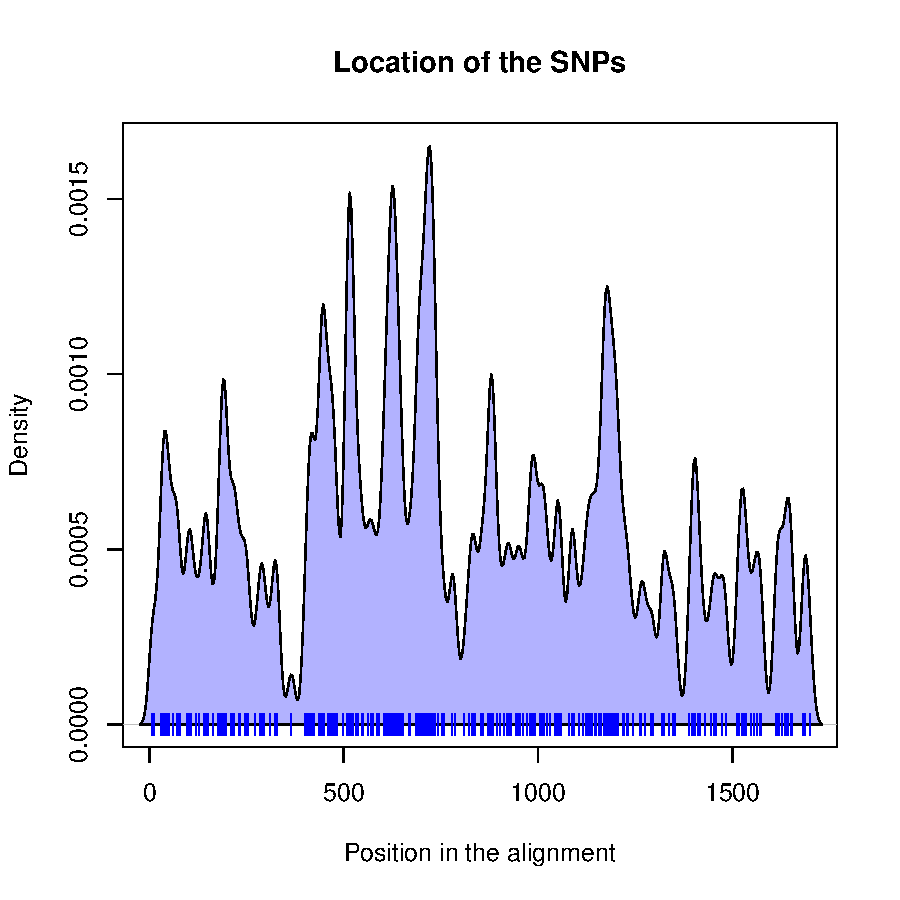
\includegraphics{figs/genomics-027}

\noindent Note that retaining only biallelic sites may cause minor loss of information, as sites
with more than 2 alleles are discarded from the data.
It is however possible to ask \texttt{fasta2genlight} to keep track of the number of alleles for
each site of the original alignment, by specifying:
\begin{Schunk}
\begin{Sinput}
> obj <- fasta2genlight(myPath, chunk = 10, saveNbAlleles = TRUE, 
+     quiet = TRUE)
> obj
\end{Sinput}
\begin{Soutput}
 === S4 class genlight ===
 80 genotypes,  274 binary SNPs
 Ploidy: 1
 26 (0 %) missing data
 @position: position of the SNPs
 @alleles: alleles of the SNPs
 @other: a list containing: nb.all.per.loc 
\end{Soutput}
\end{Schunk}

\noindent The output object \texttt{obj} now contains the number of alleles of each position, stored
in the \texttt{other} slot:
\begin{Schunk}
\begin{Sinput}
> head(other(obj)$nb.all.per.loc, 20)
\end{Sinput}
\begin{Soutput}
 [1] 1 1 1 1 1 1 2 1 1 1 1 2 1 1 1 1 1 1 1 1
\end{Soutput}
\begin{Sinput}
> 100 * mean(unlist(other(obj)) > 1)
\end{Sinput}
\begin{Soutput}
[1] 17.81305
\end{Soutput}
\end{Schunk}
About 18\% of the sites are polymorphic, which is fairly high.
This is not entirely surprising, given that the HA segment of influenza is known for its high
mutation rate.
What is the nature of this polymorphism?
\begin{Schunk}
\begin{Sinput}
> temp <- table(unlist(other(obj)))
> barplot(temp, main = "Distribution of the number \nof alleles per loci", 
+     xlab = "Number of alleles", ylab = "Number of sites")
\end{Sinput}
\end{Schunk}
Most polymorphic loci are biallelic, but a few loci with 3 or 4 alleles were lost.
We can estimate the loss of information very simply:
\begin{Schunk}
\begin{Sinput}
> temp <- temp[-1]
> temp <- 100 * temp/sum(temp)
> round(temp, 1)
\end{Sinput}
\begin{Soutput}
   2    3    4 
90.4  8.3  1.3 
\end{Soutput}
\end{Schunk}
In this case, 90.4\% of the polymorphic sites were biallelic, the others being
essentially triallelic.
This is probably a fairly exceptional situation due to the high mutation rate of the HA segment.


%% % % % % % % % % % % % % %
%% \subsubsection{Conversions within R}
%% % % % % % % % % % % % % %








%%%%%%%%%%%%%%%%
%%%%%%%%%%%%%%%%
\section{Data analysis using \texttt{genlight} objects}
%%%%%%%%%%%%%%%%
%%%%%%%%%%%%%%%%

In the following, we illustrate some methods for the analysis of \texttt{genlight} objects, ranging
from simple tools for diagnosing allele frequencies or missing data to recently developed multivariate approaches.
Troughout these examples, we use \texttt{glSim} to simulate \texttt{genlight} objects.
This simple simulation tool allows for simulating large SNPs data with possibly contrasted
structures between two groups of individuals. See \texttt{?glSim} for more details on this tool.



%%%%%%%%%%%%%%%%
\subsection{Simple operations}
%%%%%%%%%%%%%%%%





%%%%%%%%%%%%%%%%
\subsection{Principal Component Analysis (PCA)}
%%%%%%%%%%%%%%%%



%%%%%%%%%%%%%%%%
\subsection{Principal Component Analysis (PCA)}
%%%%%%%%%%%%%%%%



%%%%%%%%%%%%%%%%
\subsection{Discriminant Analysis of Principal Components (DAPC)}
%%%%%%%%%%%%%%%%







\begin{thebibliography}{9}

\bibitem{tjart05}
  Jombart, T. (2008) adegenet: a R package for the multivariate
  analysis of genetic markers. \textit{Bioinformatics} 24: 1403-1405.

\bibitem{np145}
  R Development Core Team (2011). R: A language and environment for
  statistical computing. R Foundation for Statistical Computing,
  Vienna, Austria. ISBN 3-900051-07-0.

\end{thebibliography}


\end{document}
